%% AIES submission draft, 5 October 2026.
%% Peer-review format. Do not submit the two-column option.
%% Converted from Experiments/papers/odds_ladder/w4e_odds_ladder.tex.

\documentclass{ametsocV6.2}

\title{An Evaluation Ladder for Weeks-to-Years Event Probabilities}

\authors{Dali Wang\correspondingauthor{Dali Wang, wangd@ornl.gov}\aff{a},
Daniel M. Ricciuto\aff{a},
Xiaoying Shi\aff{a},
and Deeksha Rastogi\aff{a}}

\affiliation{\aff{a}{Oak Ridge National Laboratory, Oak Ridge, Tennessee}}

\abstract{Forecast skill at leads of weeks to seasons is difficult to see in a field error.
The optimum of that error is the reference itself, so a large Earth-system model can train successfully and still leave event probabilities at their historical rate.
This paper gives a quantitative ladder for that problem.
Each rung changes one design axis: the target (an amount or a category), the season, the lead, the variable, or the object (a regional mean or a map).
Category edges and the historical class rate are fit on training time only.
A claim is kept only when the Brier skill score is positive on every held-out split.
Applied to ERA5 over the Tennessee Valley, the ladder retains winter precipitation odds out to two seasons, and one-week air-temperature and surface-runoff odds when the forecast sees the issue week's atmosphere.
Those runoff odds stay above the historical rate at two weeks and do not at three weeks.
Week-ahead rain, two- and three-week temperature, and water odds at two and three months remain at the historical rate.
The same events, edge rule, and score are the protocol for judging a coupled-model ensemble, and for judging any later artificial-intelligence model in the reanalysis world.}

\begin{document}

\maketitle

\sigstatement
A field error at leads of weeks to seasons is smallest when the forecast redraws the historical pattern.
That score can look successful while the chance of a wet, dry, hot, or cool event stays at the rate it already has.
This paper defines a ladder that changes one design choice at a time and keeps a claim only when event probabilities beat a historical rate frozen on training years, on every held-out sample.
For the Tennessee Valley in ERA5, winter precipitation and a few short-lead temperature and runoff probabilities clear that bar.
Week-ahead rain and month-ahead water odds do not.
The same bar is the test for a later artificial-intelligence model and for an Earth-system model ensemble.

\section{Introduction}
\label{sec:intro}

Leads of weeks to a few seasons sit between medium-range weather and a climate projection.
The atmospheric initial condition has mostly been lost, and a climate mean is not yet the decision~\citep{vitart2017s2s,saha2014cfsv2}.
Water availability and water temperature at that range control hydropower and thermal generation.
Physics-based systems and operational seasonal products, which are largely anomalies against a historical pattern, have limited regional skill on these decisions~\citep{saha2014cfsv2,johnson2019seas5}.
Earth-system foundation models now offer another route: transformers and diffusion ensembles trained on reanalysis or on a coupled model, often with a field loss~\citep{lam2023graphcast,bi2023pangu,nguyen2023climax,wang2024orbit}.
That loss has a known optimum.
Predicting the reference field scores well and leaves the probability of a wet, dry, hot, or cool event at the rate the event already has.

Where a predictable signal exists at these leads, it is a slow shift of that event probability away from its historical rate.
ENSO and related teleconnections are one known source of such a shift for North American precipitation~\citep{ropelewski1986enso,hong2025enso}.
A loss on amounts averages the shift away, so a network can collapse to the mean and be read as having no skill.
Extra capacity can fit weather noise and miss a shift that a small probability model still sees.
A map can be sharp and still lose to the historical field once the lead is a week.
The evaluation therefore has to be fixed before a foundation model is trained.
It has to name the event, the lead, the years that define the baseline, and the score that will count.
It has to withhold credit from a model that only redraws the reference.
The ladder in this paper is that filter.

The protocol changes one design axis at a time.
Category edges and the historical class rate are frozen from training time.
The score is the Brier skill score~\citep{brier1950,wilks2011}.
A pass is required on every pre-declared held-out split, separately for each variable and each lead.
The protocol does not depend on which world produced the sample.
The same event can be built from a reanalysis or from an Earth-system model ensemble.
Agreement across those worlds is evidence about the source of the skill.
Divergence is also a result.
The reanalysis score is not copied onto the model world.

This paper states the ladder, applies it to ERA5 over the Tennessee Valley, and writes the matched specification for a coupled-model ensemble from the Energy Exascale Earth System Model (E3SM)~\citep{hersbach2020era5,golaz2022e3sm}.
The reanalysis application is complete.
The ensemble application is the next use of the method.
A winter index gate from the same regional series is one rung of the ladder.
Its model comparison is reported separately and is not repeated here.
The contributions are the pass rule, the reanalysis claim table, and the transfer rule a later model has to meet.

\section{Evaluation Ladder}
\label{sec:method}

\subsection{One axis at a time}
\label{sec:axis}

Each rung changes one of five things: the target type (a continuous amount or a category), the season, the lead, the variable, or the forecast object (a regional mean or a map).
Predictors are a menu declared before the rung is scored.
A failure under that menu is a result for the menu.
It is not a license to search for a new predictor on the same test sample and then quote the original experiment.

\subsection{The event}
\label{sec:event}

The scored object is a regional-mean category.
For a water variable the classes are dry, near, and wet.
For temperature they are cool, near, and hot.
The two tercile edges, and the historical frequency of each class, are estimated on training time only and then frozen.
Validation and test samples are labeled with those edges.
They do not move the edges.

\subsection{The score}
\label{sec:score}

Let $p_{k,c}$ be the forecast probability of class $c$ at occasion $k$, and let $o_{k,c}$ be $1$ if that class occurs and $0$ otherwise.
The Brier score and its skill against the training class frequencies $\bar{o}_c$ are
\begin{equation}
\begin{aligned}
\mathrm{BS} &= \frac{1}{N}\sum_{k=1}^{N}\sum_{c}(p_{k,c}-o_{k,c})^{2},\\
\mathrm{BSS} &= 1 - \mathrm{BS}/\mathrm{BS}_{\mathrm{ref}},
\end{aligned}
\label{eq:bss}
\end{equation}
where $\mathrm{BS}_{\mathrm{ref}}$ uses $p_{k,c}=\bar{o}_c$~\citep{brier1950,wilks2011}.
A positive skill score means the probabilities beat that historical rate.
Hit rate and the Heidke skill score~\citep{heidke1926} are reported beside it.
A claim requires $\mathrm{BSS}>0$ on every pre-declared held-out split, for that variable and that lead.
A single season with a positive score does not replace the pooled score.
The probability model used to test the ladder is logistic regression.
It is large enough to express a shift in class probabilities and small enough that a pass is unlikely to be memorized weather.

\subsection{The baseline is declared per dataset}
\label{sec:baseline}

The historical rate in \eqref{eq:bss} is the training class frequency of the dataset being scored.
It is the baseline of that experiment.
It is not assumed to be a 30-year climate normal.
In the week and month rungs of the reanalysis case, the years that define the edges are 2010--2014, because those are the training years of the daily pack.
A new dataset names its own training years before any score is computed.
Using one normal for both a reanalysis and a coupled-model ensemble is a separate, named choice.
It is not the default here.

\subsection{Two worlds, one protocol}
\label{sec:worlds}

Observation samples and coupled-model samples may use different year lists, different ensemble sizes, and different variable names.
They use the same event definition, the same edge rule, the same score, and the same pass rule.
A pass in one world is not written into the other world's table.

\subsection{What a map may add}
\label{sec:map}

After the regional-mean probability has cleared Section~\ref{sec:score}, a map may be scored for where inside the region the event sits.
Field error at a lead is a different experiment.
A smaller field error does not clear the probability row.

\section{Reanalysis Case}
\label{sec:case}

\subsection{Region and series}
\label{sec:data}

The case is the Tennessee Valley in ERA5~\citep{hersbach2020era5}.
Seasonal rungs use a monthly index pack: autumn Pacific indices for winter precipitation, and autumn Atlantic and Arctic indices for winter air temperature, with training seasons through 2007 and 15 test seasons in 2009--2023.
Week and month rungs use daily fields on the box $34.0^{\circ}$--$37.8^{\circ}$N, $90.5^{\circ}$--$81.0^{\circ}$W.
The week split is 259 training weeks (2010--2014), 155 validation weeks (2015--2017), and 103 test weeks (2018--2019).
The month split holds out 2008 for validation and 2009--2023 for test.
These two year lists are not one sample.
Scored variables are 2~m air temperature, precipitation, and ERA5 surface runoff.
Air temperature is not river temperature.
Surface runoff is a reanalysis flux, not a stream gauge.
Figure~\ref{fig:domain} shows the seasonal predictors and the valley whose mean is the target.

\begin{figure}[!t]
\centering
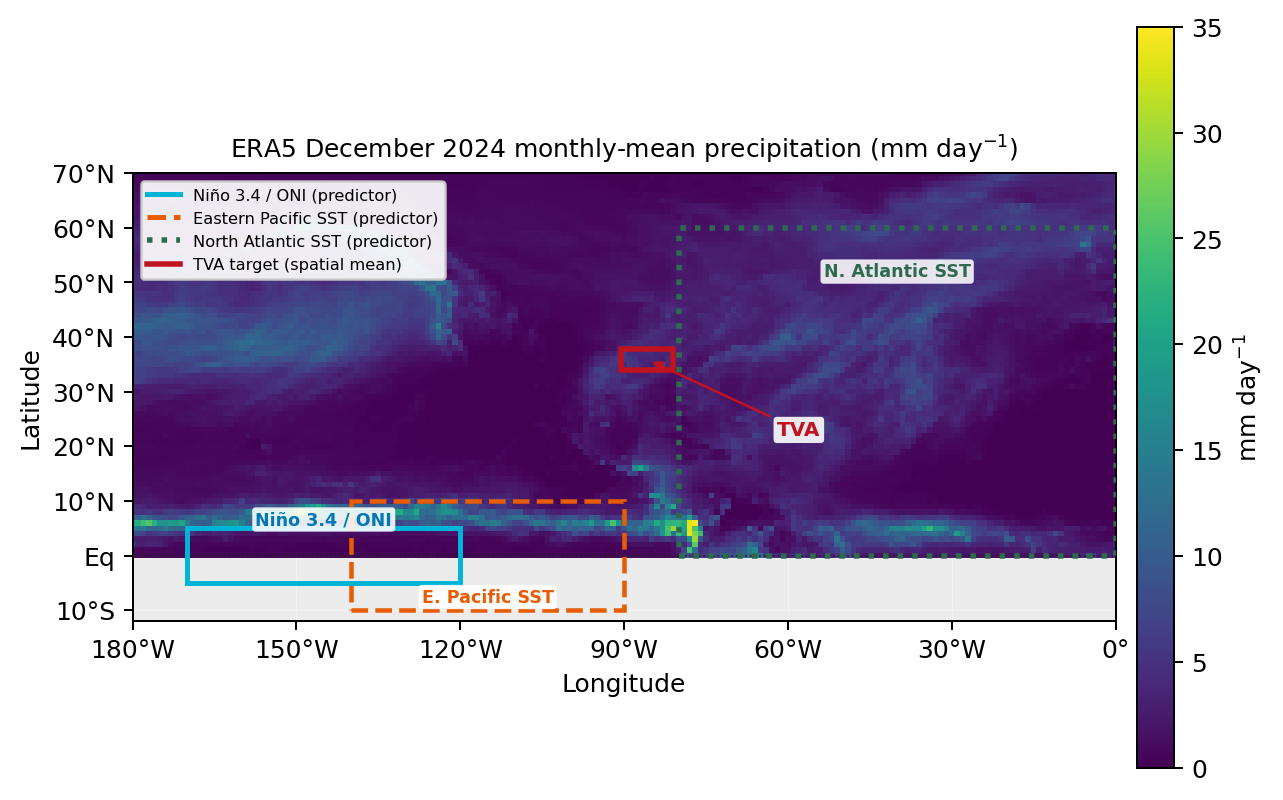
\includegraphics[width=0.92\textwidth]{figures/domain_indices_sst_tva.png}
\caption{Seasonal case geography. The red box is the Tennessee Valley mean. Pacific boxes supply the winter precipitation predictors. The North Atlantic box is the temperature-side sea-surface region. The field is one ERA5 precipitation month, shown only to locate the boxes.}
\label{fig:domain}
\end{figure}

\subsection{Rungs}
\label{sec:rungs}

Table~\ref{tab:rungs} lists the axis each rung changed.
The first rung asked whether indices forecast the monthly amount.
Subsequent rungs replaced that target with categories, then moved the season, the lead, the variable, and finally the object from a regional mean to a map.
At the week and month leads, a second logistic appends the spatial mean of the issue-period atmosphere to the indices.
That second model tests whether the recent large-scale state carries probability information beyond the slow indices.
It is still a regional-mean model.

\begin{table}[!t]

\centering
\setlength{\tabcolsep}{3pt}
\begin{tabular}{@{}p{1.55cm}p{2.15cm}p{4.0cm}@{}}
\topline
\textbf{Rung} & \textbf{Axis} & \textbf{Question} \\
\midline
Amounts & Target type & Do indices forecast the monthly amount? \\
Winter categories & Target type & Do autumn indices move winter odds? \\
Other seasons & Season & Does that menu work in spring, summer, and fall? \\
Longer winter lead & Lead & Do winter odds survive two and three seasons? \\
Maps & Object & Can a map train, and is a week-ahead rain map the product? \\
One week & Lead, variable & Do next-week odds beat the historical rate? \\
Two and three weeks & Lead & Do the one-week odds survive another one or two weeks? \\
Two and three months & Lead & Do water odds at those leads beat the historical rate? \\
Larger winter models & Capacity & Does a larger net beat the logistic on the same labels? \\
\botline
\end{tabular}
\caption{One axis changes at each rung.}
\label{tab:rungs}
\end{table}

\subsection{Seasonal categories}
\label{sec:claims}

All seasonal scores use 25 training seasons and 15 test seasons (2009--2023).
There is no separate validation year in this protocol.
Hit rate is the fraction of seasons in which the most likely class is correct.
The majority-class hit for balanced terciles is about one third.
Heidke skill corrects the hit rate for those class frequencies~\citep{heidke1926}.
Table~\ref{tab:season} applies one predictor menu to every season: autumn Pacific indices for precipitation (the Oceanic Ni\~{n}o Index and the Ni\~{n}o-3.4 region~\citep{cpc-oni,barnston1997nino34}) and autumn Atlantic and Arctic indices for temperature~\citep{hurrell1995nao,thompson1998ao}.
Winter rows are the reference rung.
The other rows change only the target season.

\begin{table}[!t]

\centering
\begin{tabular}{@{}llrrrrl@{}}
\topline
\textbf{Target} & \textbf{Event} & \textbf{Hit} & \textbf{Heidke} & \textbf{BSS} & \textbf{Majority hit} & \textbf{Result} \\
\midline
Winter & Precipitation & 0.667 & 0.432 & $+0.091$ & 0.333 & Pass \\
Winter & Air temperature & 0.400 & 0.167 & $+0.009$ & 0.133 & Pass, thin \\
Winter & Air temperature, same-season indices & 0.133 & $-0.096$ & $-0.129$ & 0.133 & Fail \\
Spring & Precipitation & 0.333 & $-0.304$ & $-0.207$ & --- & Fail \\
Spring & Air temperature & 0.133 & $-0.016$ & $-0.122$ & --- & Fail \\
Summer & Precipitation & 0.400 & 0.075 & $-0.011$ & --- & Fail \\
Summer & Air temperature & 0.333 & 0.063 & $-0.091$ & --- & Fail \\
Fall & Precipitation & 0.400 & $-0.125$ & $+0.016$ & --- & Thin \\
Fall & Air temperature & 0.400 & $-0.063$ & $-0.295$ & --- & Fail \\
\botline
\end{tabular}
\caption{Seasonal logistic odds, one season ahead, 15 test seasons. Pass requires Brier skill above zero and either Heidke skill above zero or a hit rate above the majority class.}
\label{tab:season}
\end{table}

Winter precipitation is the strong row: about two winters in three, against a one-third historical rate.
The wet/dry calls are uneven.
The model rarely selects the dry class, so the skill is a shift toward wet in some winters and toward the middle class in others.
The probability score is still the largest in the ladder.
The same Pacific predictors, scored as a continuous winter precipitation anomaly rather than a category, are only marginal (skill against the mean $+0.02$, anomaly correlation $0.44$).
Continuous winter temperature fails (skill against the mean $-0.04$).
Same-season Atlantic indices, which have no lead, also fail the winter temperature categories (BSS $-0.129$).
A contemporaneous correlation and a category forecast at a lead are different results.

Spring and summer fail for both variables.
Fall precipitation is the only non-winter positive probability score ($+0.016$), and its Heidke score is negative, so the claim is thin.
Fall temperature fails.

On the same 15 winters, October-initialized CFSv2 ensemble-mean precipitation was mapped onto the valley box and labeled with the same ERA5 terciles~\citep{saha2014cfsv2,kirtman2014nmme}.
It is correct on 7 winters (hit $0.467$, Heidke $0.111$).
The logistic is correct on 10 (hit $0.667$, Heidke $0.432$).
CFSv2 sits above the one-third majority and below the logistic.
The comparison is categorical: the ensemble mean was assigned a class, so CFSv2 has no Brier skill in this table.
Figure~\ref{fig:winter} places that comparison next to the other models trained on the same labels.
Figure~\ref{fig:cfsv2} shows why the operational hit rate stays near the majority.
The continuous October forecast is nearly flat through the test winters, while the ERA5 winter anomalies are not.
The categorical panel is the score that matches an odds product.

\begin{figure}[!t]
\centering
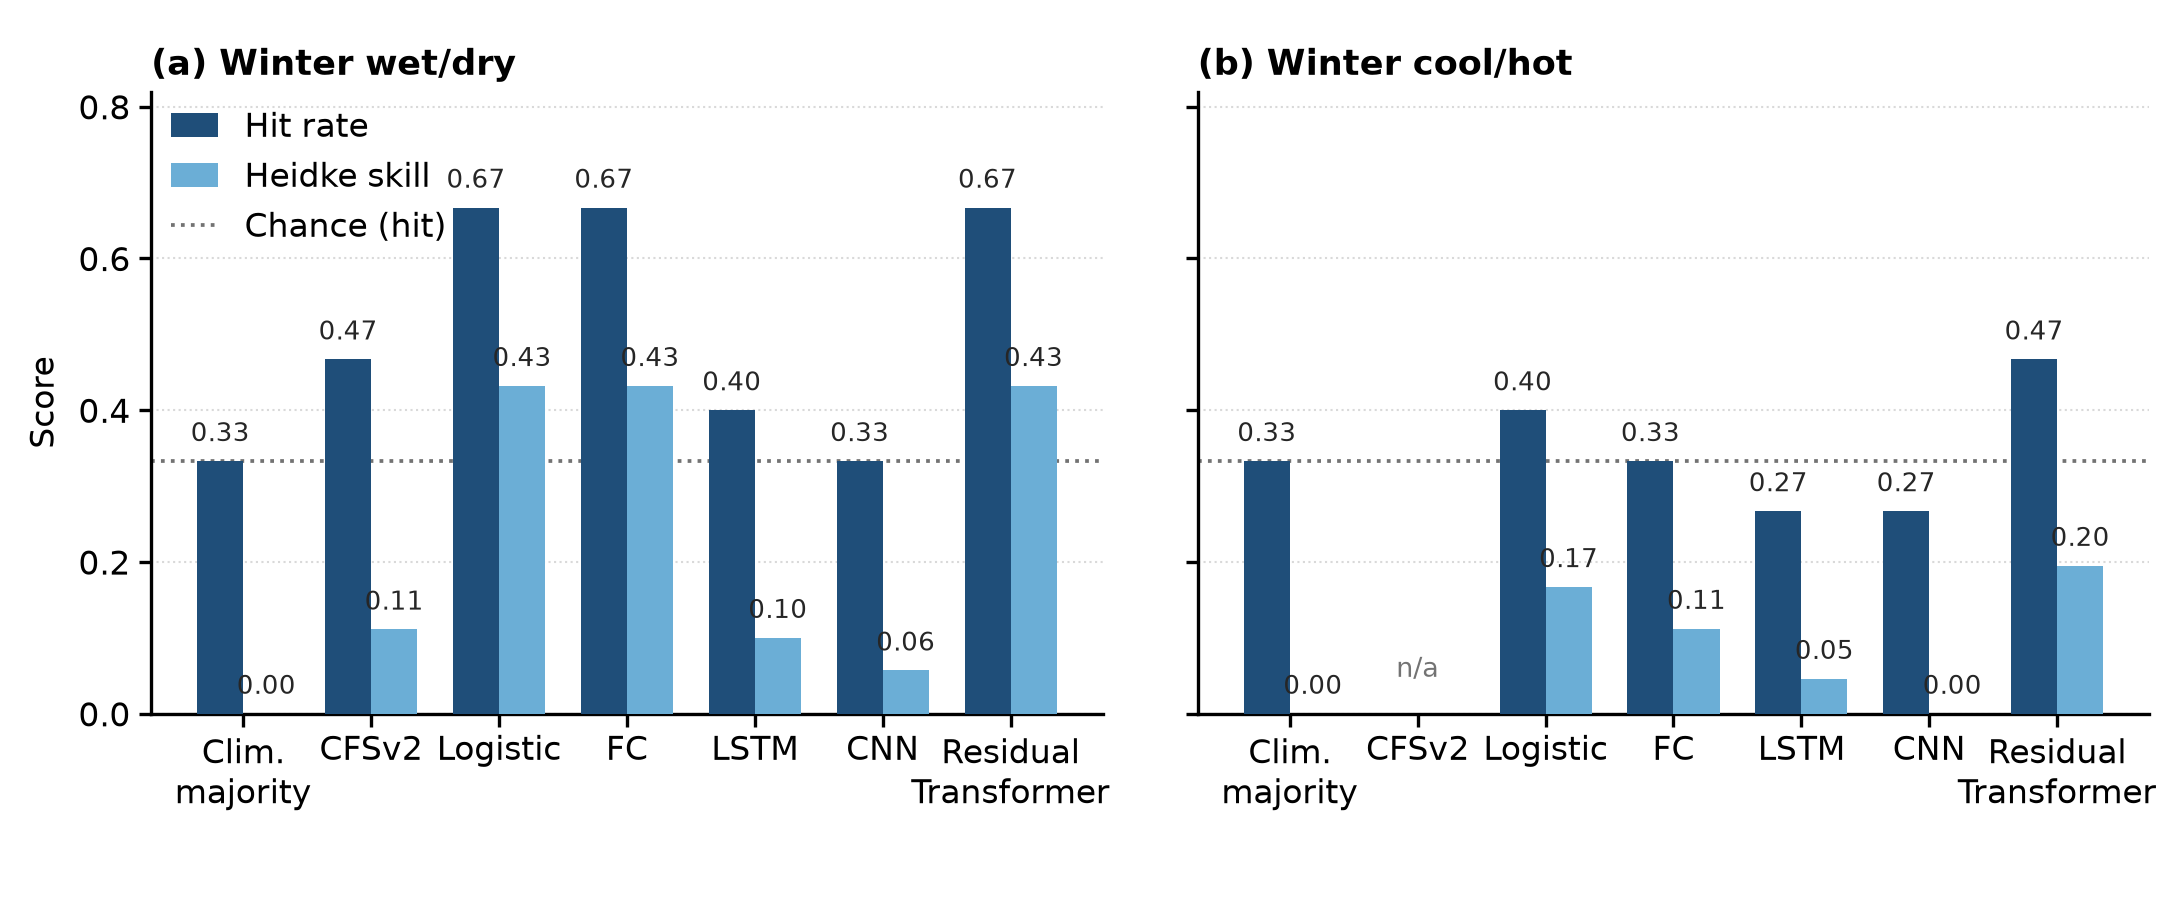
\includegraphics[width=0.92\textwidth]{figures/results_equal_panels.png}
\caption{Blocked test on 15 winters.
(a)~Winter precipitation categories, including October-initialized CFSv2 on the same ERA5 labels.
(b)~Winter temperature categories. CFSv2 was not scored on temperature.
The dotted line is a hit rate of one third.
Logistic is the reference. The residual Transformer matches its hit rate and Heidke skill on precipitation and does not classify more winters correctly.}
\label{fig:winter}
\end{figure}

\begin{figure}[!t]
\centering
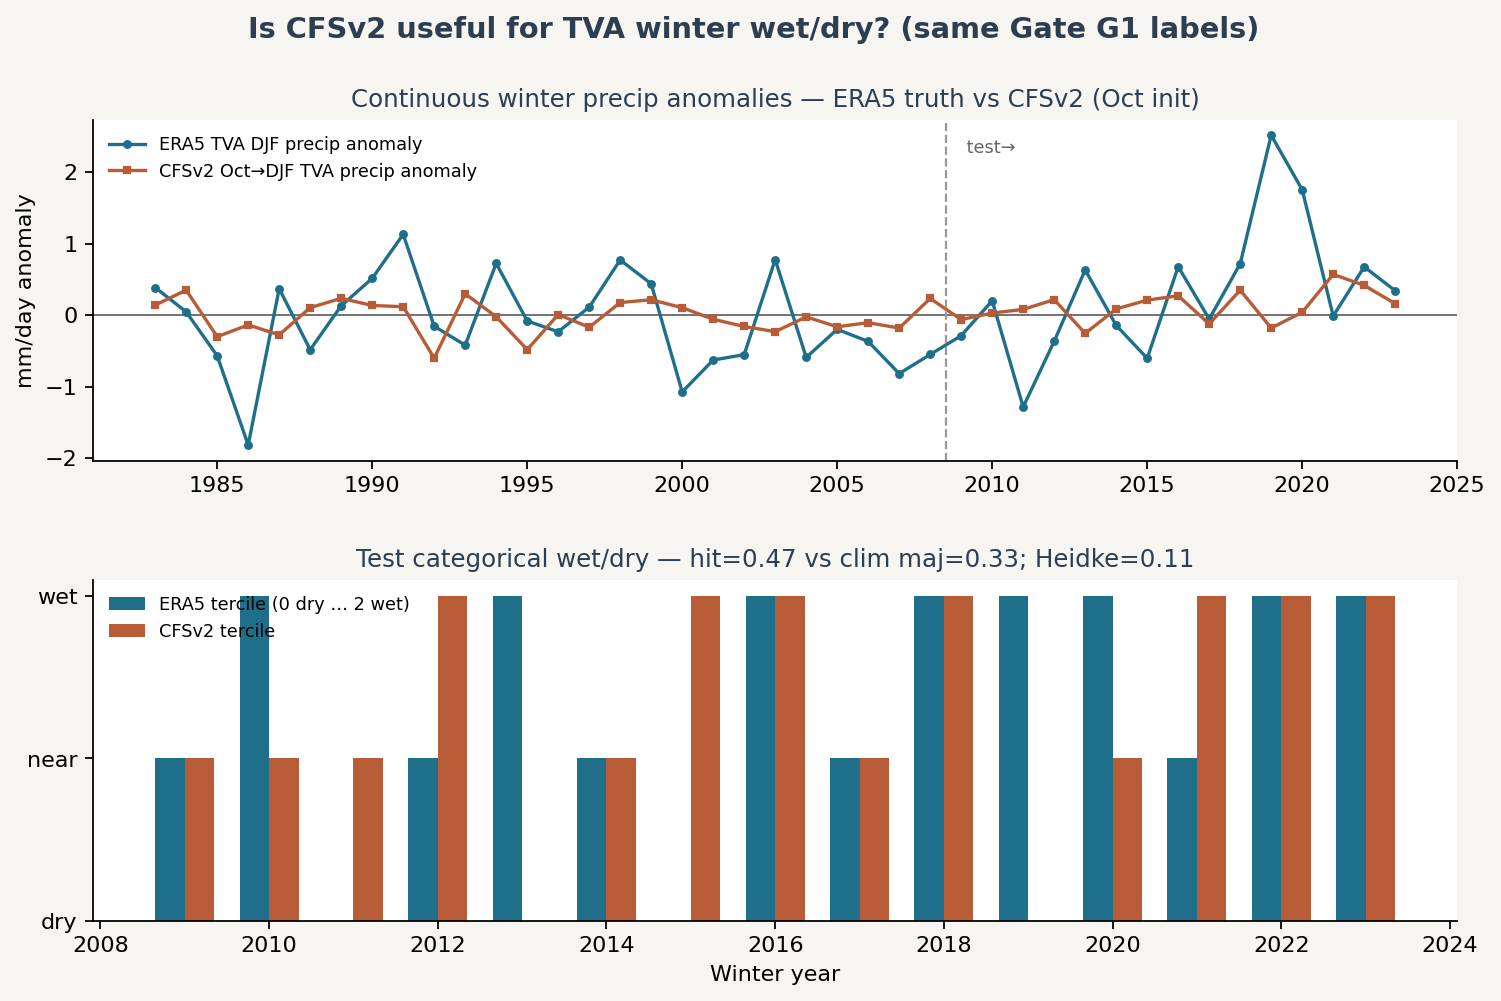
\includegraphics[width=0.78\textwidth]{figures/audience_cfsv2_g1_wetdry_scorecard.png}
\caption{October-initialized CFSv2 on the Tennessee Valley, scored against the same ERA5 winter precipitation labels as the logistic.
Top: the forecast anomaly stays near zero while the reanalysis anomaly does not.
Bottom: the resulting categories on the 15 test winters.
CFSv2 is correct on 7 winters. The logistic is correct on 10.
This is a local categorical check, not a global verification of CFSv2.}
\label{fig:cfsv2}
\end{figure}

\begin{table}[!t]

\centering
\setlength{\tabcolsep}{3pt}
\begin{tabular}{@{}llrrr@{}}
\topline
\textbf{Event} & \textbf{Model} & \textbf{Hit} & \textbf{Heidke} & \textbf{BSS} \\
\midline
Precip. & CFSv2 Oct$\rightarrow$DJF & 0.467 & 0.111 & --- \\
Precip. & Logistic & 0.667 & 0.432 & $+0.091$ \\
Precip. & Fully connected & 0.667 & 0.432 & $+0.051$ \\
Precip. & LSTM & 0.400 & 0.100 & $-0.016$ \\
Precip. & CNN & 0.333 & 0.057 & $-0.038$ \\
Precip. & Residual Transformer & 0.667 & 0.432 & $+0.140$ \\
Temp. & Logistic & 0.400 & 0.167 & $+0.009$ \\
Temp. & Residual Transformer & 0.467 & 0.195 & $+0.050$ \\
\botline
\end{tabular}
\caption{Same 15 winter test seasons. CFSv2 is an ensemble-mean class, so its Brier skill is not defined here.}
\label{tab:models}
\end{table}

The fully connected net copies the logistic hit rate and loses probability skill ($0.051$ against $0.091$).
The LSTM and the CNN fail the precipitation categories at this sample size.
The residual Transformer keeps the logistic path and adds a constrained attention correction~\citep{vaswani2017attention}.
On precipitation it matches the logistic hit and Heidke and raises Brier skill from $0.091$ to $0.140$.
On temperature it is correct on one more winter ($0.467$ against $0.400$).
It does not replace the logistic as the reference.
At the two-season precipitation lead the same style of model fell below the logistic, which is the comparison used in Table~\ref{tab:lead}.

Table~\ref{tab:lead} keeps winter as the target and moves the issue earlier.
A lead of one season reproduces the winter rows of Table~\ref{tab:season}.

\begin{table}[!t]

\centering
\setlength{\tabcolsep}{3pt}
\begin{tabular}{@{}llrrr@{}}
\topline
\textbf{Lead} & \textbf{Event} & \textbf{Hit} & \textbf{Heidke} & \textbf{BSS} \\
\midline
1 season & Precipitation & 0.667 & 0.432 & $+0.091$ \\
1 season & Air temperature & 0.400 & 0.167 & $+0.009$ \\
2 seasons & Precipitation & 0.400 & 0.135 & $+0.024$ \\
2 seasons & Air temperature & 0.267 & $-0.071$ & $-0.084$ \\
3 seasons & Precipitation & 0.133 & $-0.121$ & $-0.230$ \\
3 seasons & Air temperature & 0.200 & $-0.208$ & $-0.056$ \\
\botline
\end{tabular}
\caption{Winter odds at longer leads. Issue season is one, two, or three seasons before winter. Same 15 test winters.}
\label{tab:lead}
\end{table}

Precipitation skill falls from $+0.091$ at one season to $+0.024$ at two seasons and to $-0.230$ at three (Fig.~\ref{fig:lead}).
Temperature does not survive past one season.

\begin{figure}[!t]
\centering
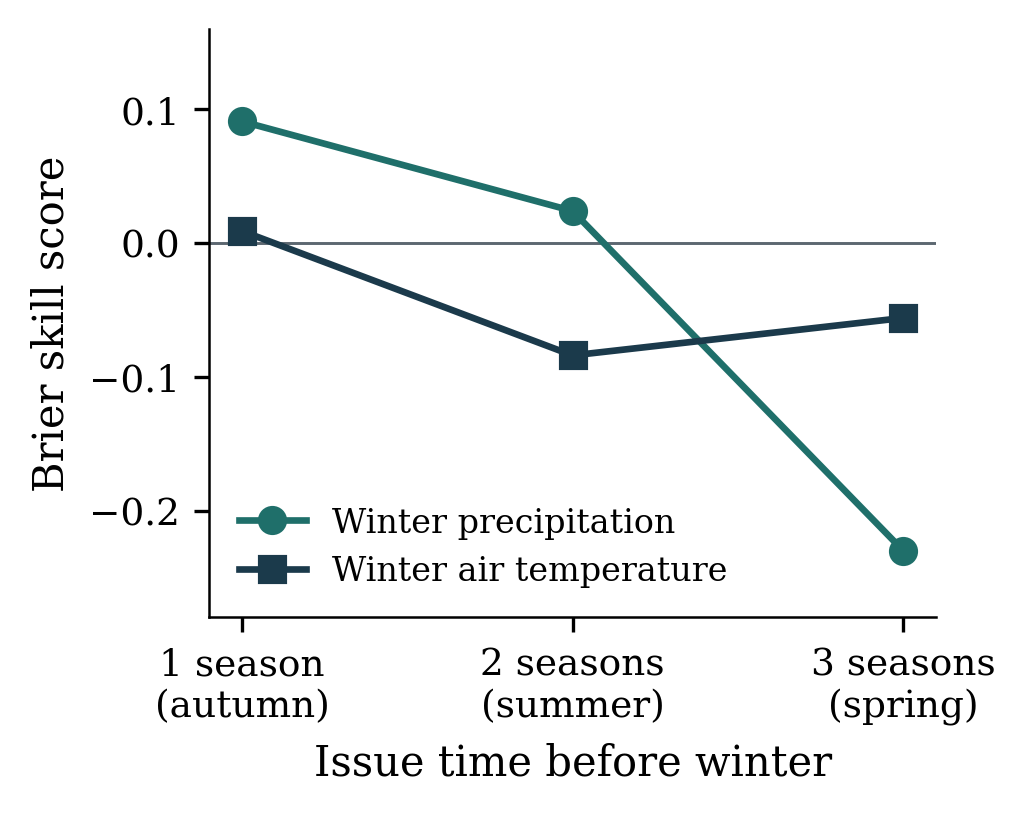
\includegraphics[width=\linewidth]{figures/fig_lead_decay.png}
\caption{Winter category skill as the issue moves earlier. Above zero beats the historical class rate. Precipitation remains positive at two seasons and fails at three.}
\label{fig:lead}
\end{figure}
The logistic remains the reference at both leads, including after the model comparison in Table~\ref{tab:models}.
Table~\ref{tab:claims} collects the claim that follows from Tables~\ref{tab:season} and~\ref{tab:lead}.

\begin{table}[!t]

\centering
\setlength{\tabcolsep}{3pt}
\begin{tabular}{@{}p{3.4cm}p{2.6cm}p{3.4cm}l@{}}
\topline
\textbf{Event} & \textbf{Lead} & \textbf{Held-out BSS} & \textbf{Claim} \\
\midline
Winter precip. & 1 season & $+0.091$ & yes \\
Winter air temp. & 1 season & $+0.009$ & thin \\
Fall precip. & 1 season & $+0.016$ & thin \\
Winter precip. & 2 seasons & $+0.024$ & thin \\
Week air temp. & 1 week & $+0.018/+0.032$ & yes \\
Week runoff & 1 week & $+0.018/+0.052$ & yes \\
Week runoff & 2 weeks & $+0.033/+0.014$ & thin \\
Week precip.; month water & 1 week; 2--3 mo & Tables~\ref{tab:week}--\ref{tab:month} & no \\
Other 2--3 week rows & 2--3 weeks & Table~\ref{tab:week2} & no \\
\botline
\end{tabular}
\caption{Claims retained from the reanalysis case. Thin means a small positive Brier skill, or a positive Brier skill with a negative Heidke score.}
\label{tab:claims}
\end{table}

\subsection{One week ahead}
\label{sec:week}

The week rung uses the next ISO week after the issue Sunday.
Training, validation, and test contain 259, 155, and 103 weeks.
A pass requires Brier skill above zero on both the validation weeks and the test weeks.
Table~\ref{tab:week} separates indices at the issue Sunday from the same indices plus the spatial mean of that week's $1^{\circ}$ atmosphere (temperature, precipitation, and sea-level pressure) and the month of the year.
Summer and winter columns are slices of the test set.
They are reported so a pooled pass can be read by season.
They are not a substitute for the pooled pass.

\begin{table}[!t]

\centering
\begin{tabular}{@{}llrrrr@{}}
\topline
\textbf{Variable} & \textbf{Predictors} & \textbf{Val} & \textbf{Test} & \textbf{Test summer} & \textbf{Test winter} \\
\midline
Air temperature & Indices & $-0.114$ & $-0.040$ & $+0.063$ & $-0.101$ \\
Air temperature & Indices $+$ atmosphere & $+0.018$ & $+0.032$ & $+0.212$ & $-0.119$ \\
Precipitation & Indices & $-0.003$ & $+0.031$ & $-0.007$ & $+0.066$ \\
Precipitation & Indices $+$ atmosphere & $-0.003$ & $+0.066$ & $+0.031$ & $+0.176$ \\
Surface runoff & Indices & $-0.005$ & $+0.024$ & $-0.005$ & $+0.053$ \\
Surface runoff & Indices $+$ atmosphere & $+0.018$ & $+0.052$ & $+0.077$ & $+0.078$ \\
\botline
\end{tabular}
\caption{One-week Brier skill for the Tennessee Valley mean. Indices alone fail every variable. The atmosphere column adds the issue-week spatial mean.}
\label{tab:week}
\end{table}

Two rows pass.
Air temperature with the issue-week atmosphere is positive on validation ($+0.018$) and on test ($+0.032$).
The test skill is in summer ($+0.212$).
Test winter is negative ($-0.119$), so this is not a winter temperature forecast.
Surface runoff with the same predictors is positive on validation ($+0.018$) and on test ($+0.052$), and the test summer and test winter slices are both positive ($+0.077$ and $+0.078$).
Hit rates on the test weeks for these two passing models are $0.47$ for temperature and $0.45$ for runoff.
Precipitation with the atmosphere reaches $+0.066$ on the test weeks, including $+0.176$ in test winter, and remains negative on validation ($-0.003$).
The pass rule therefore rejects week-ahead precipitation.
Figure~\ref{fig:week} is that comparison.
The right-hand season panel is not the pass rule.
It shows where the test skill sits: temperature skill is in summer, and winter temperature is negative.

\begin{figure}[!t]
\centering
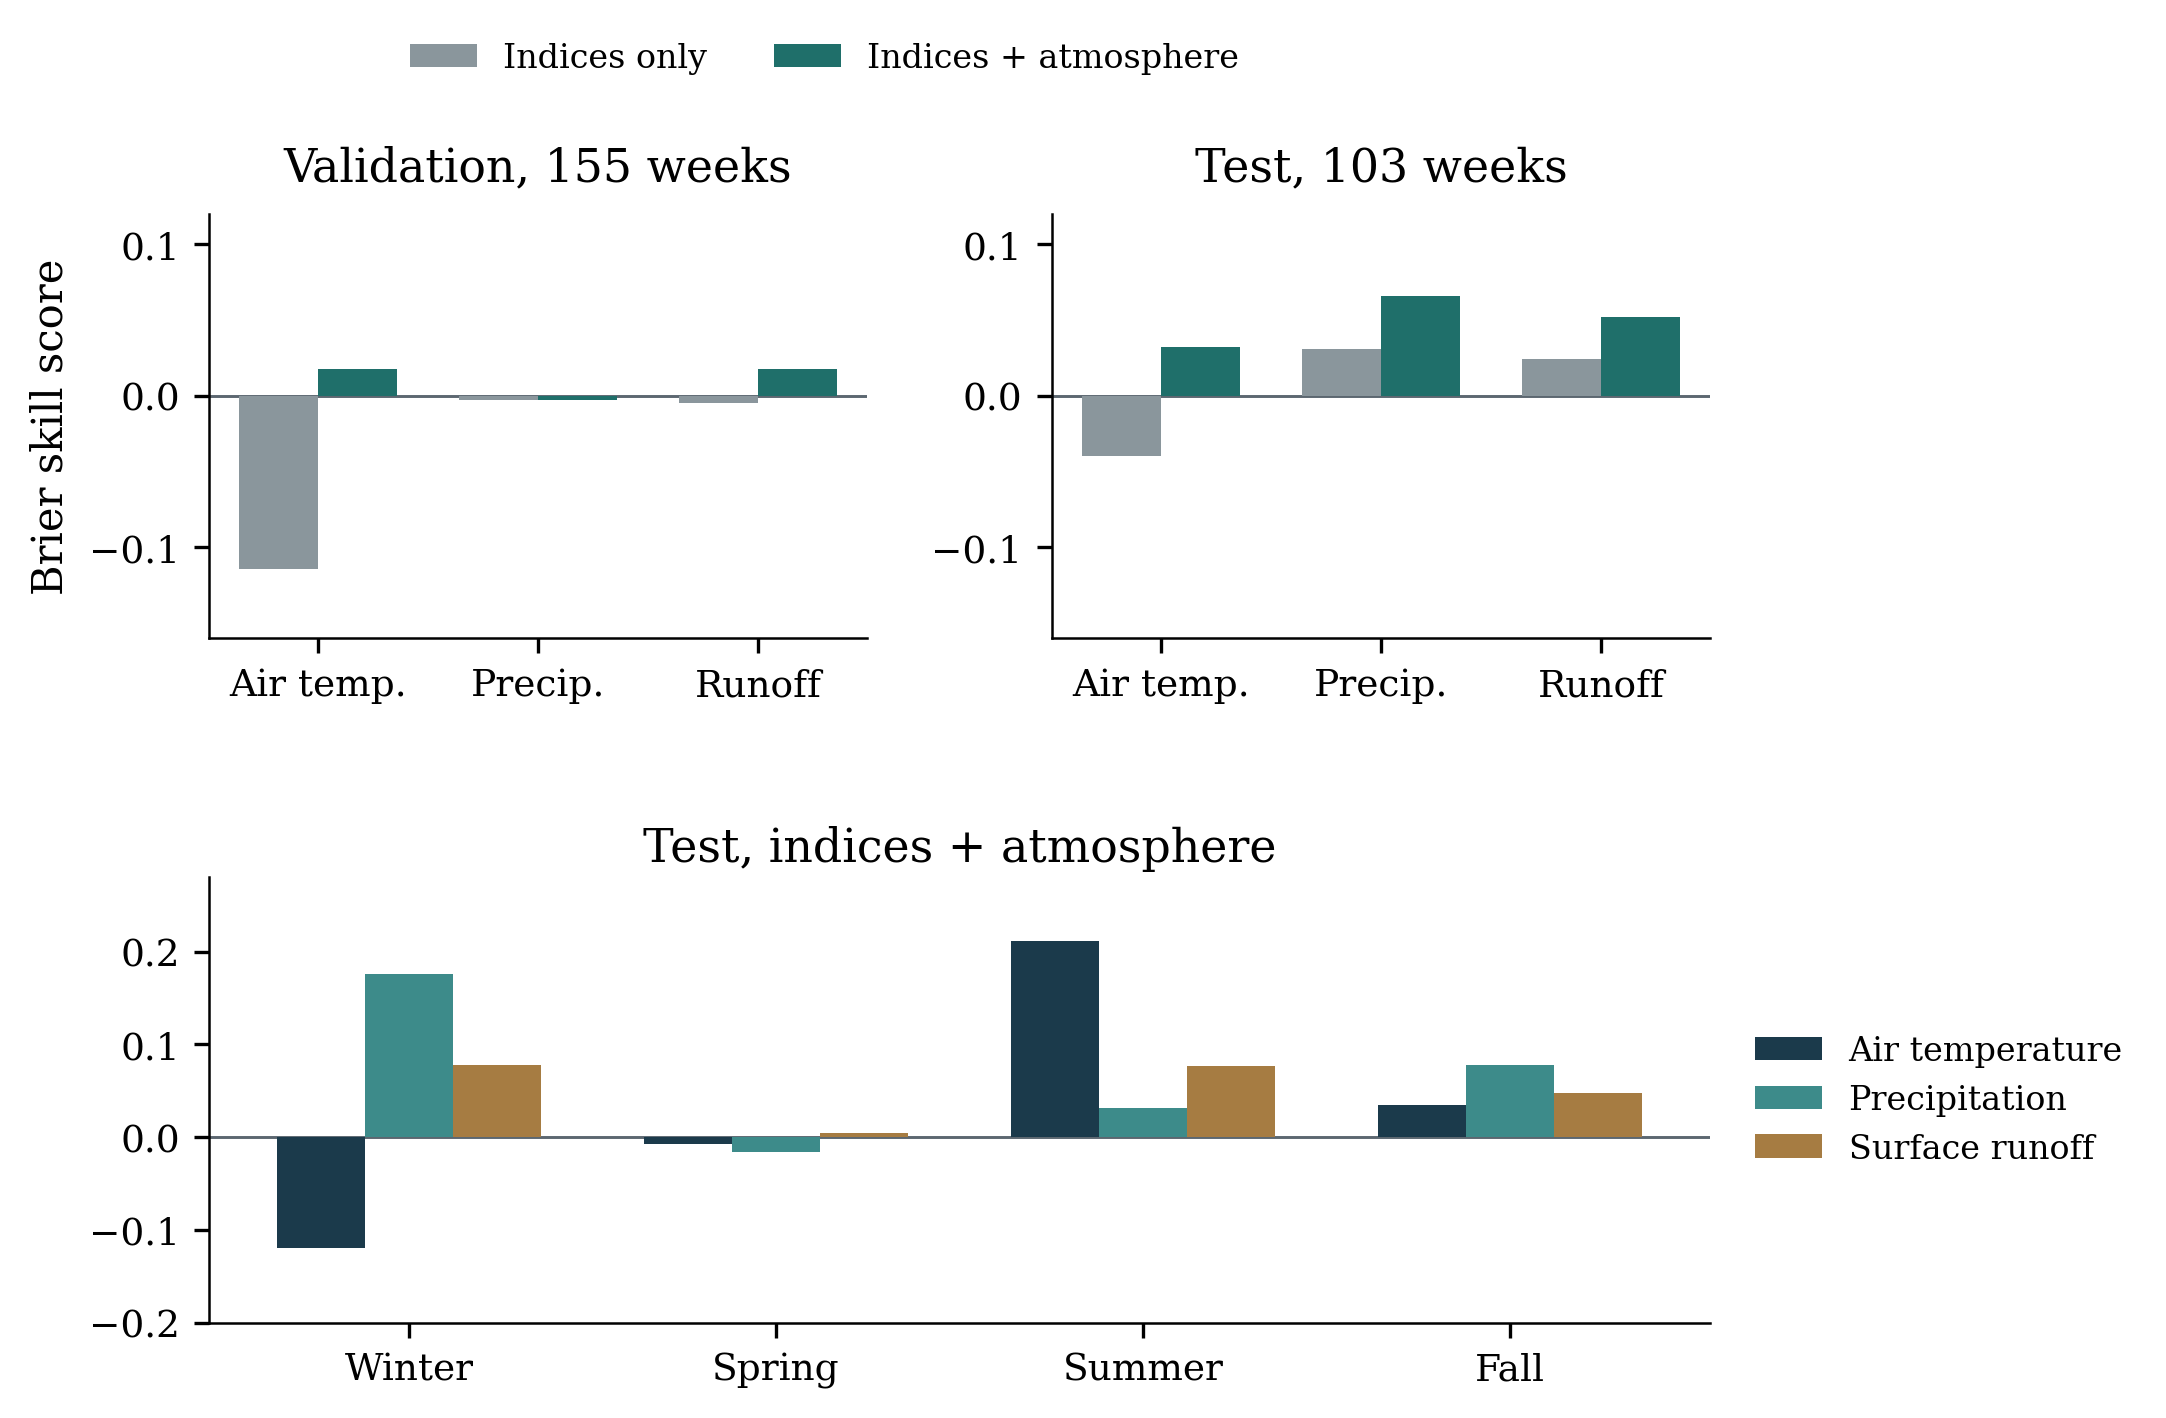
\includegraphics[width=\textwidth]{figures/fig_week_bss.png}
\caption{One-week Brier skill for the valley mean.
Left and center: indices alone against indices plus the issue week's atmosphere.
A pass requires both of those panels to be above zero.
Right: the passing predictor set, split by season on the test weeks.}
\label{fig:week}
\end{figure}
The same week list, scored as precipitation amount maps rather than as odds, loses to the historical field: root-mean-square error $0.64$ for the map model and $0.53$ for the historical map.

\subsection{Two and three weeks ahead}
\label{sec:week23}

The longer week leads use the same issue weeks and the same two logistics.
The target is the valley mean two ISO weeks ahead, and, in a separate fit, three ISO weeks ahead.
Issue-time predictors stay on the issue week.
Tercile edges are refit on that lead's training weeks.
A row is dropped when the target week is not in the same split as the issue week, so lead $+2$ has 258, 154, and 102 weeks and lead $+3$ has 257, 153, and 101.
Table~\ref{tab:week2} is the same pass rule as Table~\ref{tab:week}.

\begin{table}[!t]

\centering
\setlength{\tabcolsep}{3.5pt}
\begin{tabular}{@{}llrrrrc@{}}
\topline
\textbf{Lead} & \textbf{Predictors} & \textbf{Val} & \textbf{Test} & \textbf{Test summer} & \textbf{Test winter} & \textbf{Pass} \\
\hline
\multicolumn{7}{@{}l}{\emph{Air temperature}} \\
$+2$ weeks & Indices & $-0.106$ & $-0.037$ & $+0.052$ & $-0.103$ & no \\
$+2$ weeks & Indices $+$ atmosphere & $-0.060$ & $-0.026$ & $+0.166$ & $-0.158$ & no \\
$+3$ weeks & Indices & $-0.097$ & $-0.037$ & $+0.051$ & $-0.086$ & no \\
$+3$ weeks & Indices $+$ atmosphere & $-0.055$ & $-0.043$ & $+0.147$ & $-0.190$ & no \\
\multicolumn{7}{@{}l}{\emph{Precipitation}} \\
$+2$ weeks & Indices & $-0.005$ & $+0.015$ & $-0.000$ & $+0.038$ & no \\
$+2$ weeks & Indices $+$ atmosphere & $-0.003$ & $+0.009$ & $+0.013$ & $+0.106$ & no \\
$+3$ weeks & Indices & $-0.019$ & $-0.015$ & $+0.004$ & $-0.025$ & no \\
$+3$ weeks & Indices $+$ atmosphere & $-0.038$ & $-0.025$ & $+0.011$ & $+0.045$ & no \\
\multicolumn{7}{@{}l}{\emph{Surface runoff}} \\
$+2$ weeks & Indices & $-0.007$ & $+0.021$ & $-0.008$ & $+0.035$ & no \\
$+2$ weeks & Indices $+$ atmosphere & $+0.033$ & $+0.014$ & $+0.055$ & $+0.030$ & thin \\
$+3$ weeks & Indices & $-0.010$ & $+0.009$ & $-0.017$ & $+0.016$ & no \\
$+3$ weeks & Indices $+$ atmosphere & $-0.008$ & $-0.040$ & $+0.035$ & $-0.019$ & no \\
\botline
\end{tabular}
\caption{Two- and three-week Brier skill for the Tennessee Valley mean. Each lead is a separate logistic with its own terciles. One row passes.}
\label{tab:week2}
\end{table}

One row clears the bar.
Surface runoff at two weeks, with the issue-week atmosphere, is positive on validation ($+0.033$) and on test ($+0.014$).
Test summer and test winter are both positive ($+0.055$ and $+0.030$).
Test fall is $-0.030$ and validation fall is $-0.011$.
The hit rate on the 102 test weeks is $0.40$ and the Heidke score is $+0.12$.
The skill is smaller than the one-week runoff row, and Table~\ref{tab:claims} marks it thin.
Temperature at both longer leads keeps a positive test-summer slice and a negative test-winter slice, and the pooled scores are negative.
Two-week precipitation reaches $+0.106$ in test winter and remains negative on validation ($-0.003$).
At three weeks, no variable is positive on both splits.

\subsection{Two and three months ahead}
\label{sec:month}

The month rung uses every issue month from August 1982 through January 2023 (486 months).
Training runs through December 2007 (305 months), validation is calendar 2008 (12 months), and the test is January 2009 through January 2023 (169 months).
Leads of two and three months are fit separately, with separate tercile edges.
Table~\ref{tab:month} is Brier skill for precipitation and surface runoff.
Persistence, a hard bet on the class of the issue month, is worse than the historical rate throughout this table, often with skill near $-1$.
It is not a useful null at these leads.

\begin{table}[!t]

\centering
\begin{tabular}{@{}llrrrrr@{}}
\topline
\textbf{Lead} & \textbf{Model} & \textbf{Val} & \textbf{Test} & \textbf{Test summer} & \textbf{Test winter} & \textbf{Pass} \\
\hline
\multicolumn{7}{@{}l}{\emph{Precipitation}} \\
$+2$ months & Indices & $-0.005$ & $-0.006$ & $-0.008$ & $-0.015$ & no \\
$+2$ months & Indices $+$ atmosphere & $-0.055$ & $-0.031$ & $-0.028$ & $-0.032$ & no \\
$+3$ months & Indices & $+0.021$ & $-0.007$ & $+0.001$ & $-0.009$ & no \\
$+3$ months & Indices $+$ atmosphere & $-0.022$ & $-0.034$ & $-0.019$ & $-0.014$ & no \\
\multicolumn{7}{@{}l}{\emph{Surface runoff}} \\
$+2$ months & Indices & $+0.055$ & $-0.004$ & $-0.023$ & $+0.006$ & no \\
$+2$ months & Indices $+$ atmosphere & $-0.056$ & $-0.001$ & $+0.031$ & $+0.032$ & no \\
$+3$ months & Indices & $+0.033$ & $+0.002$ & $-0.006$ & $-0.001$ & no \\
$+3$ months & Indices $+$ atmosphere & $-0.162$ & $-0.049$ & $-0.009$ & $+0.009$ & no \\
\botline
\end{tabular}
\caption{Month-ahead Brier skill. Each lead is a separate logistic. The atmosphere column adds the issue-month spatial mean and made every test score worse.}
\label{tab:month}
\end{table}

No cell clears the pass rule once summer and winter are both required to be positive.
Three-month runoff with indices alone is the only pooled test score above zero, at $+0.002$, after a positive validation score of $+0.033$.
Its test summer slice is $-0.006$ and its test winter slice is $-0.001$.
The pooled value is a residual across seasons, not a winter signal and not a summer signal, and it is not entered as a claim in Table~\ref{tab:claims}.
The atmospheric mean lowers the test skill in every row, including that one.
Figure~\ref{fig:month} shows the index-only test scores, which are the stronger of the two models.
The pooled three-month runoff bar is the only one above zero, and its summer and winter slices are not.

\begin{figure}[!t]
\centering
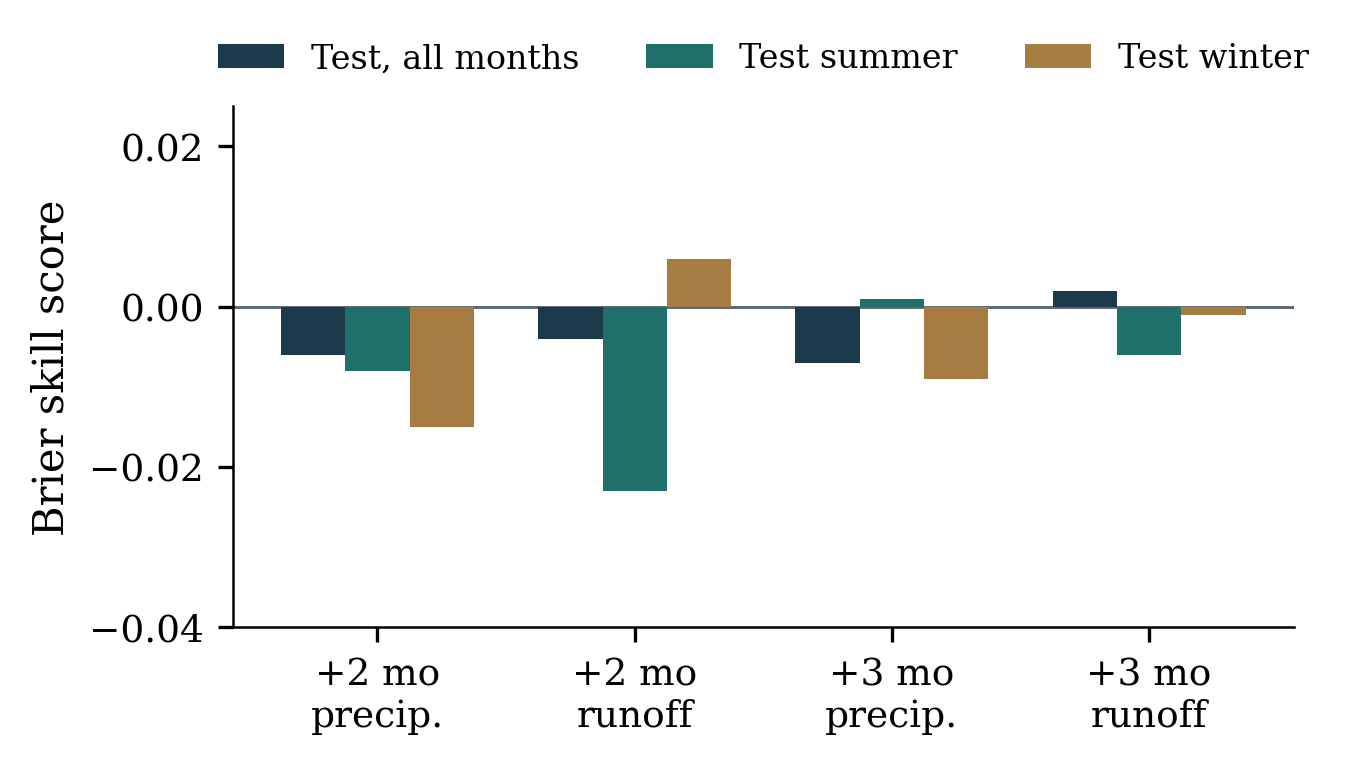
\includegraphics[width=\linewidth]{figures/fig_month_bss.png}
\caption{Month-ahead water odds from indices alone, on the 169 test months.
The scale is a few hundredths of a Brier skill point.
No lead is positive in both summer and winter.}
\label{fig:month}
\end{figure}

\subsection{What the failures fix in the score}
\label{sec:failures}

The opening amount model used this month calendar and a masked squared error on standardized anomalies at leads of one to three months together.
It scored near the long-term average and stopped at the first epoch.
That run is why Tables~\ref{tab:season}--\ref{tab:month} score categories rather than amounts.
Same-day maps can be trained on this archive, so a map failure at a lead is not a pipeline failure.
Same-day surface runoff is readable from the atmosphere.
Top-layer soil moisture is not, and soil moisture was left off the probability gate.
Week-ahead rain maps and week-ahead rain probabilities fail together.
On the winter labels, extra capacity raised the one-season probability score once and lost to the logistic at two seasons.
The event definition, not the size of the network, is what separates the rows that pass from the rows that do not.

\section{Using the Ladder Again}
\label{sec:again}

\subsection{A later model in the same reanalysis}
\label{sec:later}

A later model trained on these fields is scored by reducing it to Table~\ref{tab:claims}.
The reduction uses the same issue times, the same regional mean, and the same frozen edges.
Where the claim is ``yes'' or ``thin,'' the regional-mean probabilities have to beat the logistic skill on that row, on the same held-out splits.
Where the claim is ``no,'' the floor is the historical rate in \eqref{eq:bss}.
A spatial probability map is scored after that regional mean has cleared the row.
The week-ahead rows and the seasonal rows are different events.
Passing one does not pass the other.
A two-week runoff probability has to beat the two-week logistic in Table~\ref{tab:week2}.
Temperature and precipitation at two weeks, and every variable at three weeks, have no passing logistic.
Their floor is the historical rate.
A weekly reference map that the model displays, including a multi-decade week-of-year mean, is not the tercile ruler of Section~\ref{sec:baseline}.
Scoring against a newly chosen normal is a new case.

\subsection{Transfer to a coupled-model ensemble}
\label{sec:e3sm}

The same ladder is the test of predictability inside E3SM~\citep{golaz2022e3sm}.
The scientific question is whether the events in Table~\ref{tab:claims} shift, at the same leads, in the coupled model, and where the two worlds diverge.
Table~\ref{tab:transfer} states what is shared and what is recomputed.
The ensemble this specification is written for is the subseasonal-to-decadal set with starts on 1~May and 1~November, 1980--2013, members EN00--EN09.
Those starts are not the 2010--2014 reanalysis weeks.
Tercile edges are fit on the ensemble's own training starts.

\begin{table}[!t]

\centering
\setlength{\tabcolsep}{3pt}
\begin{tabular}{@{}p{2.2cm}p{5.5cm}@{}}
\topline
\textbf{Piece} & \textbf{Rule} \\
\midline
Events & Regional-mean dry/near/wet or cool/near/hot, at the leads already tested: one, two, and three weeks; two and three months; one to three seasons. \\
Edges & Terciles from that world's training sample only. \\
Score & Brier skill \eqref{eq:bss} on held-out samples, per variable and per lead, positive on every declared split. \\
Comparison & Each cell is reported against Table~\ref{tab:claims}. Either world may pass while the other fails. \\
Fields & Declared before scoring. Air temperature $\leftrightarrow$ \texttt{TREFHT} or \texttt{TBOT}; precipitation $\leftrightarrow$ \texttt{PRECT} or \texttt{RAIN}+\texttt{SNOW}; surface runoff $\leftrightarrow$ \texttt{QOVER}, with \texttt{QRUNOFF} only if the surface flux is absent. \\
\botline
\end{tabular}
\caption{What transfers to a second world. Years, edges, and field names are recomputed. The event, the edge rule, and the score are shared.}
\label{tab:transfer}
\end{table}

The field names are a translation, not a result.
This paper stops at the specification.
The ensemble scorecard is a later measurement.

\section{Limitations}
\label{sec:limits}

Fifteen test seasons can support a research gate.
They cannot support an operational hit-rate claim.
The winter precipitation model rarely calls the dry class, so the probability score is the more stable summary.
Validation at the month lead is a single year.
The week split and the seasonal split cover different years, and a sentence that merges them is not supported.
The 2010--2014 terciles are the training ruler of the week and month rungs, not a named climate normal.
A failed season is a result for the pre-declared index menu.
Air temperature and surface runoff are proxies for the thermal and water events that matter to energy operations.
The coupled-model application has no score until that ensemble is run through Section~\ref{sec:e3sm}.
The CFSv2 comparison is a Tennessee Valley categorical check on 15 winters~\citep{barnston2012cfsv2}.
It is not a global verification of that forecast system.

\section{Conclusion}
\label{sec:conc}

Weeks-to-years event probabilities are a hard forecast problem because a field error is minimized by redrawing the reference.
The ladder isolates the alternative quantity: a shift of category probabilities above a historical rate that was frozen before the test.
In ERA5 over the Tennessee Valley the filter keeps winter precipitation odds out to two seasons, one-week air-temperature and surface-runoff odds when the issue week's atmosphere is included, and a thinner two-week surface-runoff odds from those same predictors.
It rejects three-week odds, week-ahead precipitation, and the two- and three-month water rows.
A later model in this reanalysis is an advance only when its regional-mean probabilities beat that table.
An E3SM ensemble is judged by the same events and the same score, on edges fit to its own training starts.

\clearpage
\acknowledgments
This research was supported by the U.S. Department of Energy Genesis Mission / Water4Energy project (DE-FOA-0003612).
It used resources of the Oak Ridge Leadership Computing Facility, a DOE Office of Science User Facility.
This manuscript has been authored by UT-Battelle, LLC, under contract DE-AC05-00OR22725 with the U.S. Department of Energy.
The U.S. government retains a nonexclusive, paid-up, irrevocable, worldwide license to publish or reproduce the published form of this manuscript, or allow others to do so, for U.S. government purposes.
DOE will provide public access to these results in accordance with the DOE Public Access Plan (\url{http://energy.gov/downloads/doe-public-access-plan}).
The authors declare no conflicts of interest.

\availstatement
The seasonal rungs use the monthly AI-ready pack archived at \url{https://doi.org/10.13139/ORNLNCCS/3409936}.
The week and month scorecards that support the tables (\texttt{bandw\_odds\_scorecard.json}, \texttt{bandw\_leads23\_scorecard.json}, and \texttt{bandm\_odds\_scorecard.json}) and the script that scores the two- and three-week leads accompany this manuscript.
ERA5 is the Copernicus reanalysis described by \citet{hersbach2020era5}.

\clearpage
\bibliographystyle{ametsocV6}
\bibliography{references}

\end{document}
